\documentclass[10pt,a4paper, margin=1in]{article}
\usepackage{fullpage}
\usepackage{amsfonts, amsmath, pifont}
\usepackage{amsthm}
\usepackage{graphicx}
\usepackage{float}
\usepackage{listings}
\usepackage{tkz-euclide}
\usepackage{tikz}
\usepackage{pgfplots}
\pgfplotsset{compat=1.13}

\usepackage{geometry}
 \geometry{
 a4paper,
 total={210mm,297mm},
 left=10mm,
 right=10mm,
 top=10mm,
 bottom=10mm,
 }
 % Write both of your names here. Fill exxxxxxx with your ceng mail address.
 \author{
  İşleyici, Osman Taylan\\
  \texttt{e2448496@ceng.metu.edu.tr}
  \and
  Deveci, Cengizhan\\
  \texttt{e2448322@ceng.metu.edu.tr}
}

\title{CENG 384 - Signals and Systems for Computer Engineers \\
Spring 2023 \\
Homework 4}
\begin{document}
\maketitle



\noindent\rule{19cm}{1.2pt}

\begin{enumerate}

    \item %write the solution of q1
          \begin{enumerate}
              % Write your solutions in the following items.
              \item~\\
              $\frac{Y(jw)}{X(jw)} = H(jw) = \frac{jw-1}{jw+1}$\\
              $Y(jw)(jw+1) = X(jw)(jw-1)$\\
              If we take the inverse fourier transform of both sides;\\
              $\dot{y}(t)+y(t) = \dot{x}(t)-x(t)$ is our differential equation.
              \item~\\
              $H(jw) = 1-\frac{2}{jw+1}$\\ If we take the inverse fourier transform using the table;\\
              $h(t) = \delta(t) - 2e^{-t}u(t)$.
              \item~\\
              The output can be found by concatanating input and impulse response;\\
              $y(t) = e^{-2t}u(t)\ast(\delta(t)-2e^{-t}u(t))$\\
              If we take the fourier transform of this equation;\\
              $Y(jw) = \frac{jw-1}{(jw+2)\cdot(jw+1)}$\\
              $Y(jw) = \frac{A}{jw+2}+\frac{B}{jw+1}$\\
              $Y(jw) = \frac{3}{jw+2} - \frac{2}{jw+1}$\\
              Now we can inverse fourier transform this equation to find $y(t)$.\\
              $y(t) = 3e^{-2t}u(t) - 2e^{-t}u(t)$.\\
              \begin{tikzpicture}
                  \draw[->] (-3,0) -- (7,0) node[right] {$t$};
                  \draw[->] (0,-2) -- (0,3) node[above] {$y$};

                  \draw[domain=0:7,smooth,variable=\t,blue] plot ({\t},{3*exp(-2*\t) - 2*exp(-\t)});
                  \node[blue,right] at (5.8,0.4) {$3e^{-2t}u(t)-2e^{-t}u(t)$};
              \end{tikzpicture}
              \item~\\
              \begin{center}
                  \tikzset{%
                      block/.style    = {draw, thick, rectangle, minimum height = 3em,
                              minimum width = 3em},
                      sum/.style      = {draw, circle, node distance = 2cm}, % Adder
                      input/.style    = {coordinate}, % Input
                      output/.style   = {coordinate} % Output
                  }
                  % Defining string as labels of certain blocks.
                  \newcommand{\suma}{\Large$+$}
                  \newcommand{\inte}{$\displaystyle \int$}
                  \newcommand{\derv}{\huge$\frac{d}{dt}$}

                  \begin{tikzpicture}[auto, thick, node distance=2cm, >=triangle 45]
                      \draw
                      % Drawing the blocks of first filter :
                      node at (0, 0) [input] (inp) {\Large \textopenbullet}
                      node [output, right of = inp] (out1) {}
                      node [output, below of = out1] (out2) {}
                      node [block, right of = out2] (derv1) {\derv}
                      node [output, right of = derv1] (out3) {}
                      node [sum, above of = out3] (sum1) {\suma}
                      node [sum, right of = out1] (sum2) {\suma}
                      node [output, right of = sum1](out4) {}
                      node [output, right of = out4](y){}
                      node [output, above of = out4](out5){}
                      node [block, left of = out5](derv2){\derv}
                      node [output, left of = derv2] (out6) {}
                      % node [sum, right of=inp] (sum) {\suma}
                      % node [block, right of=sum] (int) {\inte}
                      % node [output, right of=int] (out) {}
                      % node [output, right of=out] (out2) {\Large \textopenbullet}
                      % node [output, below of=out] (temp1) {}
                      % node [output, below of=sum] (temp2) {}
                      ;
                      \draw[-](inp) -- node{$x(t)$}(out1);
                      \draw[-](out1) -- (out2);
                      \draw[->](out2)--(derv1);
                      \draw[-](derv1) -- (out3);
                      \draw[->](out3) -- (sum1);
                      \draw[->](out1)--node{$-1$}(sum2);
                      \draw[->](sum2)--(sum1);
                      \draw[-] (sum1)--(out4);
                      \draw[->] (out4)--node{$y(t)$}(y);
                      \draw[-] (out4)--(out5);
                      \draw[->] (out5)--(derv2);
                      \draw[-] (derv2) -- node{$-1$}(out6);
                      \draw[->] (out6)--(sum2);
                      % \draw[->](inp) -- node{$x(t)$} (sum);
                      % \draw[->](sum) -- (int);
                      % \draw[-](int) -- (out);
                      % \draw[->](out) -- node{$y(t)$} (out2);
                      % \draw[-](out) -- (temp1);
                      % \draw[->](temp2) -- (sum);
                      % \draw[-](temp1) -- node{$-5$} (temp2);
                  \end{tikzpicture}
              \end{center}
          \end{enumerate}




    \item %write the solution of q2  
          \begin{enumerate}
              % Write your solutions in the following items.
              \item %write the solution of q2a
              $y[n+1] \leftrightarrow^F e^{jw}Y(e^{jw})$ \\

              $y[n] \leftrightarrow^F Y(e^{jw})$ \\

              $x[n+1] \leftrightarrow^F e^{jw}X(e^{jw})$ \\

              $e^{jw} Y(e^{jw}) - \frac{1}{2} Y(e^{jw}) = e^{jw} X(e^{jw})$\\

              $Y(e^{jw}) (e^{jw} - \frac{1}{2}) = e^{jw} X(e^{jw })$ \\

              $\frac{Y(e^{jw})}{X(e^{jw})} = H(e^{jw}) = \frac{e^{jw}}{e^{jw} - \frac{1}{2}}$ \\

              \item %write the solution of q2b
            
              $\frac{e^{jw}}{e^{jw}(1 - \frac{1}{2} e^{-jw})} = \frac{1}{1 - \frac{1}{2}e^{-jw}}$ \\

              $(\frac{1}{2})^n u[n] \leftrightarrow \frac{1}{1 - \frac{1}{2}e^{-jw}}$ \\

              $h[n] = (\frac{1}{2})^n u[n]$

              \item %write the solution of q2c
              
              $(\frac{3}{4})^nu[n] \leftrightarrow \frac{1}{1-\frac{3}{4}e^{-jw}}$ \\

              $Y(e^{jw}) = X(e^{jw}) H(e^{jw})$ \\

              from part a and b we know $H(e^{jw}) = \frac{1}{1-\frac{1}{2}e^{-jw}}$ \\

              $Y(e^{jw}) = \frac{1}{1-\frac{3}{4}e^{-jw}} \frac{1}{1-\frac{1}{2}e^{-jw}} = \frac{A}{1-\frac{3}{4}e^{-jw}} + \frac{B}{1-\frac{1}{2}e^{-jw}}$\\

              $A (1-\frac{1}{2}e^{-jw}) + B(1-\frac{3}{4}e^{-jw}) = 1$\\

              $A - A\frac{1}{2}e^{-jw} + B - \frac{3}{4}e^{-jw} = 1$\\

              $A+B = 1 $ and $\frac{A}{2} + \frac{3B}{4} = 0$ \\

              $A = 3$ and $B = -2$\\

              $Y(e^{jw}) = \frac{3}{1 - \frac{3}{4}e^{-jw}} - \frac{2}{1 - \frac{1}{2}e^{-jw}}$ \\

              $y[n] = (3(\frac{3}{4})^2 - 2(\frac{1}{2})^n)u[n]$


          \end{enumerate}

    \item %write the solution of q3
          \begin{enumerate}
              % Write your solutions in the following items.
              \item~\\
              $\frac{Y(jw)}{X(jw)}=H(jw)=H_1(jw)\cdot H_2(jw)$\\
              $\frac{Y(jw)}{X(jw)} = \frac{1}{(jw+1)\cdot(jw+2)}$\\
              $=\frac{1}{(jw)^2+3jw+2}$\\
              $Y(jw)((jw)^2+3jw+2) = X(jw)$\\
              We inverse fourier transform this equation and get;\\
              $\ddot{y}(t)+3\dot{y}(t)+2y(t) = x(t)$\\
              \item~\\Inverse fourier transform of $H(jw)$;\\
              $H(jw) = \frac{1}{jw+1} - \frac{1}{jw+2}$\\
              $h(t) = e^{-t}u(t) -e^{-2t}u(t)$\\
              \item~\\ $\frac{Y(jw)}{X(jw)} = H(jw)$\\
              $\rightarrow Y(jw) = \frac{jw}{(jw+1)(jw+2)}$\\
              $\rightarrow Y(jw) = \frac{A}{jw+1} + \frac{B}{jw+2}$\\
              $Y(jw) = \frac{2}{jw+2} - \frac{1}{jw+1}$\\
              Inverse fourier transform of $Y(jw)$ gives us $y(t)$.\\
              $y(t) = 2e^{-2t}u(t)-e^{-t}u(t)$\\
          \end{enumerate}

    \item %write the solution of q4
          \begin{enumerate}
              % Write your solutions in the following items.
              \item %write the solution of q4a
              $Y(e^{jw}) = X(e^{jw}) H_1(e^{jw}) + X(e^{jw}) H_2(e^{jw})$ \\

              $\frac{Y(e^{jw})}{X(e^{jw})} = H(e^{jw}) = H_1(e^{jw}) + H_2(e^{jw}) = \frac{1}{1 + \frac{1}{3}e^{-jw}} + \frac{1}{1 + \frac{1}{2}e^{-jw}}$ \\

              $H(e^{jw}) = \frac{1 + \frac{1}{2}e^{-jw} + 1 + \frac{1}{3}e^{-jw}}{(1 + \frac{1}{3}e^{-jw})(1 + \frac{1}{2}e^{-jw})}.$ \\

              $= \frac{2 + \frac{5}{6} e^{-jw}}{1+ \frac{5}{6}e^{-jw}+\frac{1}{6}(e^{-jw})^2} = \frac{12 + 5e^{-jw}}{6+5e^{-jw}+(e^{-jw})^2}$ \\

              $Y(e^{jw}) (6+5e^{-jw}+(e^{-jw})^2) = X(e^{jw}) (12 + 5e^{-jw})$ \\

              $Y(e^{jw}) (e^{-jw})^2 + Y(e^{jw}) 5e^{-jw}+ 6Y(e^{jw}) = X(e^{jw}) 5e^{-jw}+ 12X(e^{jw})$ \\

              $y[n-2] + 5y[n-1] +6y[n] = 5x[n-1] + 12x[n]$
            
              \item %write the solution of q4b
              $Y(e^{jw}) = X(e^{jw}) H_1(e^{jw}) + X(e^{jw}) H_2(e^{jw})$ \\

              $\frac{Y(e^{jw})}{X(e^{jw})} = H(e^{jw}) = H_1(e^{jw}) + H_2(e^{jw}) = \frac{1}{1 + \frac{1}{3}e^{-jw}} + \frac{1}{1 + \frac{1}{2}e^{-jw}}$ \\
              \item %write the solution of q4c
              We can find the h[n] by using Fourier Transform. \\
              $(\frac{-1}{3})^nu[n] \leftrightarrow \frac{1}{1 + \frac{1}{3}e^{-jw}}$ \\
              
              and \\

              $(\frac{-1}{2})^nu[n] \leftrightarrow \frac{1}{1 + \frac{1}{2}e^{-jw}}$ \\

              $h[n] = (\frac{-1}{2})^nu[n] + (\frac{-1}{3})^nu[n]$

          \end{enumerate}

    \item ~\\
          The secret message is; \textbf{I have a dream.}\\
          \begin{figure}[H]
            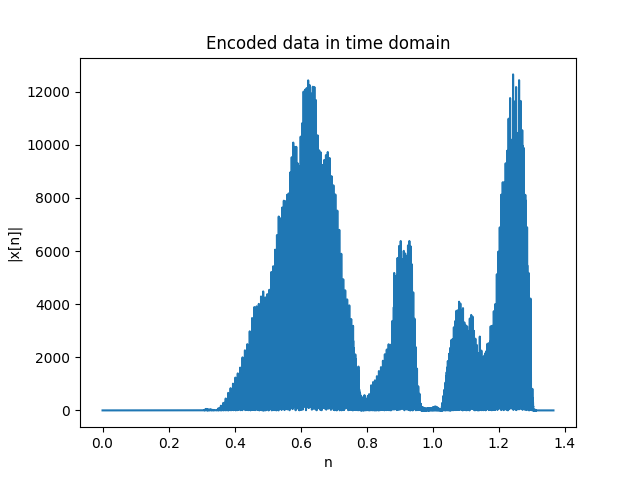
\includegraphics[scale = 0.75]{e_t}
            \caption{Magnitude of encoded data in time domain.}
          \end{figure}~\\
          \begin{figure}[H]
            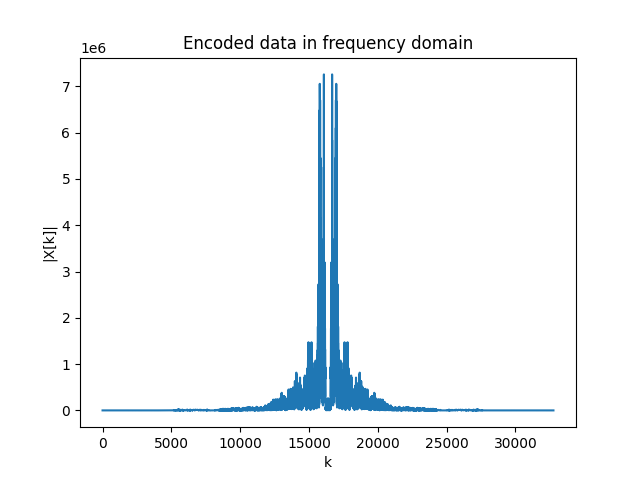
\includegraphics[scale = 0.75]{e_f}
            \caption{Magnitude of encoded data in frequency domain.}
          \end{figure}~\\
          \begin{figure}[H]
            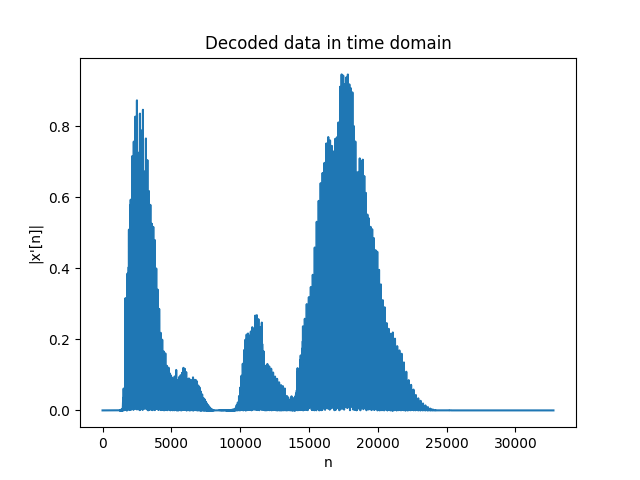
\includegraphics[scale = 0.75]{d_t}
            \caption{Magnitude of decoded data in time domain.}
          \end{figure}~\\
          \begin{figure}[H]
            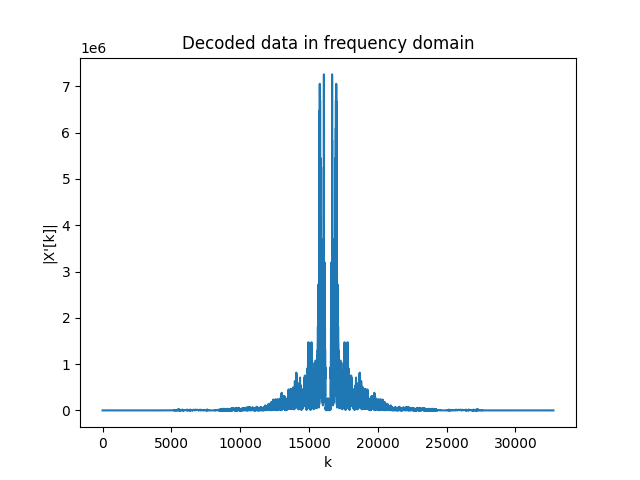
\includegraphics[scale = 0.75]{d_f}
            \caption{Magnitude of decoded data in frequency domain.}
          \end{figure}~\\
          \lstset{language=Python}
    \lstset{frame=single}
    \lstset{caption={Solution code}}
    \lstset{label={lst:code_direct}}
    \lstset{basicstyle=\footnotesize}
    \begin{lstlisting}
        import numpy as np
        import matplotlib.pyplot as plt
        import scipy.io as sio
        
        
        def fft(signal):
            N = len(signal)
            if N <= 1:
                return signal
        
            # dividing signal into two parts and fft'ing them
            evenPart = fft(signal[::2])
            oddPart = fft(signal[1::2])
        
            fourierTransform = np.zeros(N, dtype=np.complex128)
            for i in range(N // 2):
                oddPart_i = oddPart[i] * np.exp(-2j * np.pi * i / N)
                fourierTransform[i] = evenPart[i] + oddPart_i
                fourierTransform[i + N // 2] = evenPart[i] - oddPart_i
            return fourierTransform
        
        
        def ifft(signal):
            csignal = np.conjugate(signal)
            return np.conjugate(fft(csignal))/len(signal)
        
        
        def plotter(data, title, xlabel, ylabel):
            plt.figure()
            plt.plot(np.abs(data))
            plt.title(title)
            plt.ylabel(ylabel)
            plt.xlabel(xlabel)
        
        
        def decode(rate, data):
            # plot original data in time domain
            plotter(data, "Encoded data in time domain", "n", "|x[n]|")
        
            # fourier transforming data
            fourierTransformed = fft(data)
            plotter(fourierTransformed,
                    "Encoded data in frequency domain", "k", "|X[k]|")
        
            # dividing data to positive and negative part
            firstHalf = fourierTransformed[:len(data)//2]
            secondHalf = fourierTransformed[len(data)//2:]
        
            # concatanating them
            reversedAndConcatenated = np.concatenate(
                [firstHalf[::-1], secondHalf[::-1]])
        
            # inverse fft
            newData = ifft(reversedAndConcatenated)
        
            # normalizing
            decoded = np.real(newData)/np.max(np.abs(newData))
            plotter(decoded, "Decoded data in time domain", "n", "|x'[n]|")
        
            # normalizing and writing to file.
            sio.wavfile.write('decodedOutput.wav', rate, decoded)
            return data
        
        
        def main():
            # reading rate and data
            rate, data = sio.wavfile.read("encoded.wav")
            decoded = decode(rate, data)
            fourierOfDecoded = fft(decoded)
            plotter(fourierOfDecoded, "Decoded data in frequency domain", "k", "|X'[k]|")
            plt.show()
            """Secret message is I have a Dream."""
        
        
        if __name__ == "__main__":
            main()
        
                        
    \end{lstlisting}


\end{enumerate}


\end{document}

